
%%%%%%%%%%%%%%%%%%%%%%%%%%%%%%%%%%%%%%%%%%%%%%%%%%%%%%%%%%%%%%%%%%%%%%%%%%%%%%%%%%%%%%%%%%%%%
%%									ANNEXES 											    	  %
%%%%%%%%%%%%%%%%%%%%%%%%%%%%%%%%%%%%%%%%%%%%%%%%%%%%%%%%%%%%%%%%%%%%%%%%%%%%%%%%%%%%%%%%%%%%%

\selectlanguage{french} %ou english
\chapter{Informations supplémentaires pour le chapitre \ref{chap:experimentation}}  \label{secanchap4}


%\minitoc
%\recto


%%%%%%%%%%%%%%%%%%%%%%%%%%%%%%%%%%%%%%%%%%%%%%%%%%%%%%%%%%%%%%%%%%%%%%%%%%%%%%%%%%%%%%%%%%%%%

	
\section{Production de larves  \textit{Meloidogyne  incognita}} \label{secan1}


\hspace{-8mm}
	  \includegraphics[scale=0.8]{protocoleA}
     
        
        
\noindent \textbf{ \underline{Objectif} }: production massive de larves de nématodes du genre \textit{Meloidogyne}.

\noindent \textbf{ \underline{Protocoles cités} }: protocole PROT-BIOL-N4 « Extraction des œufs de \textit{ Meloidogyne}  et éclosion en condition quasi
\og stérile \fg .

\noindent \textbf{ \underline{Matériels et réactifs} }:

\vspace{-5mm}
\begin{minipage}[c]{0.85 \linewidth}
		\begin{itemize}[leftmargin=0cm]
		\item racines lavées de tomates infestées avec galles et masses d'œufs apparentes,
		\item seaux de 5 litres percés à 2 cm du fond, 
		\item tamis à mailles de  \SI{10}{\micro\metre} .
		 \end{itemize}
\end{minipage}
 \hspace{3mm}
\begin{minipage}{0.5 \textwidth}
		\begin{figure}[H]          
		\includegraphics[width=0.5\textwidth]{tamis}  
			\begin{minipage}{0.5 \textwidth}
			\caption{ tamis à mailles de  \SI{10}{\micro\metre} et 1 mm}
			\label{tamis}
			\end{minipage} 
	    \end{figure}
\end{minipage} 
        
        
\noindent \textbf{ \underline{Hygiène et Sécurité} } : aucun risque. 

\noindent \textbf{ \underline{Déroulement de l'expérience} } : 


\begin{itemize}[ label=\ding{172}]
\item les racines de tomate (\textit{Solanum lycopersicum}) de la variété Saint Pierre (variété sensible aux nématodes)  
     inoculées préalablement (1,5 mois à 25$^{\circ}$ C) sont récoltées après l'apparition de galles formées de masses    
     d’œufs. Par la suite, les racines sont  soigneusement
     lavées.
\end{itemize}

\begin{itemize}[ label=\ding{173}]
\item Les racines de tomates sensibles inoculées sont récupérées, coupées, broyées 1 minute  dans une solution de javel 
    (NaOCI) à 1 \%. Ce traitement a pour effet de libérer les œufs enveloppés dans une gangue
	gélatineuse. Ces œufs sont répartis dans des éclosoirs  contenant des  tamis à maille de 10 \si{\micron}
	(\autoref{tamis}). Les tamis sont posés sur de l'eau aérée par système de bulleur (type bulleur d'aquarium).
\end{itemize}

\begin{itemize}[ label=\ding{174}]
\item  Les larves juvéniles de deuxième stade (J2s) qui  émergent traversent  ce tamis à maille de 10  \si{\micron} et
	se retrouvent en suspension dans l'eau (\autoref{J2}).  Ceci permet de récupérer
	500 J2 dans 1 ml de solution pour effectuer les tests d’infestation. La première récolte de larves dans l’eau se 
	fait après une semaine. Elles
	peuvent se conserver une semaine à 4$^{\circ}$ C. En outre,   pour réaliser une bonne inoculation, il est 
	préférable de sortir les larves du frigo et de les
	laisser 2 à 3 heures à température ambiante avant de commencer les infestations. Néanmoins, l'idée du stockage des 
	larves est une solution alternative. Il est préférable d'utiliser des larves fraîches pour faire les inoculations. 
	Des larves de J2 fraîchement écloses (24-48h maximum) en suspension dans l'eau sont utilisées pour des inoculations 
	des plantes.
\end{itemize}

\begin{figure}[H]
	\centering \includegraphics[scale=0.5]{J2_oeufsA.pdf}
	\caption[ (A) Larves en suspension dans l’eau et (B) œufs libérés de la masse
     	mucilagineuse entourant la ponte.]{ \textbf{A} Larves en suspension dans l’eau et \textbf{B} œufs libérés de la 
	    masse mucilagineuse entourant la ponte par
	    vortexage 10 mn dans une solution de javel à 1 \% de chlore actif.}
    \label{J2}
\end{figure}


	
\section[Quantification du nombre de nématodes dans la plante]{Quantification du nombre de nématodes à galles (du genre \textit{Meloidogyne}) dans la plante} \label{secan2}


\hspace{-8mm}

\includegraphics[scale=0.8]{protocoleB}
             
\noindent \textbf{ \underline{Objectif} }: Quantifier le nombre de nématodes à galles (\textit{Meloidogyne spp.}) dans la plante.

\noindent \textbf{ \underline{Protocoles cités} }: protocole PROT-BIOL-N7  \og Coloration des masses d’œufs de \textit{Meloidogyne spp.} (coloration à l’éosine) pour comptage \fg .


\noindent \textbf{ \underline{Matériels et réactifs} }:
\begin{itemize}
\item chambre climatique  (cycle des nématodes = 35 environs  à 24$^{\circ}$C),
\item  pots de dimension  9x9x9,
\item sol sableux stérile (470 g par pot),
\item tomates sensibles aux nématodes, St Pierre par exemple (une plante par pot), 
\item pour quantification précise des nématodes : 
{\small \begin{enumerate}
\item[$\bullet$] poudre d’éosine B,  
\item[$\bullet$] 1 bouteille en verre ou plastique pour conserver la solution à 1g/l à température ambiante,  
\item[$\bullet$] récipients de 1 litre type bécher.
\end{enumerate}}
\end{itemize}


 
\noindent \textbf{ \underline{Déroulement de l'expérience} } : 


\begin{description}
\item[jour J0] : semis de 40 plantes de tomates en pots.

\item[J+ 42 jours] : 4 modalités d'inoculation par plante : 0, 433, 5784 et 11568 J2, soit un total d'environs 150 000 J2.

\item[J + 77 jours] :
	{\small \begin{itemize}[itemsep=15pt, topsep=5pt]
	\item après un cycle du nématodes de 35 jours à 24$^{\circ}$C. Arracher les tomates numérotés selon la dose 
	      d'inoculation, éliminer les partie aériennes, rincer délicatement les racines à l'eau (\autoref{racines}),\\
		\begin{minipage}[c]{0.70 \textwidth}
				\begin{figure}[H]     
				\centering \includegraphics[width=1\textwidth]{racines}
				\caption{ Racines de tomates numérotés selon la dose d'inoculation initiale.}
				\label{racines}
				\end{figure}
		\end{minipage}
	\item compter le nombre de pontes en les colorant à l’éosine (PROT-BIOL-N7): \\
	      Chaque ponte correspond à 1 nématode ayant pénétré dans la racine (\autoref{eosine}). 
		   \begin{minipage}[c]{0.70 \textwidth}
			   \begin{figure}[H]     
			   \centering \includegraphics[width=1\textwidth]{eosine}
			   \caption{ Coloration des  racines de tomates à l’éosine.}
			   \label{eosine}
			   \end{figure}
		\end{minipage}
	\end{itemize}}

\end{description}



\iffalse
\includepdf[scale=0.9, pages=1,pagecommand=\section{Les systèmes de cultures du Projet SMaCH GEDUNEM} \label{secan3}
,offset=0 -1.5cm]{Djian_Caporalino2019_ProjetSMaCH_GEDUNEM.pdf}
\includepdf[scale=0.9,pages=2-6,pagecommand={},offset=0 0.5cm]{Djian_Caporalino2019_ProjetSMaCH_GEDUNEM.pdf}
\fi
	
\section{Figure supplémentaire pour le chapitre \ref{chapter4}}  \label{secan4}

		\begin{figure}[H]
		\centering
			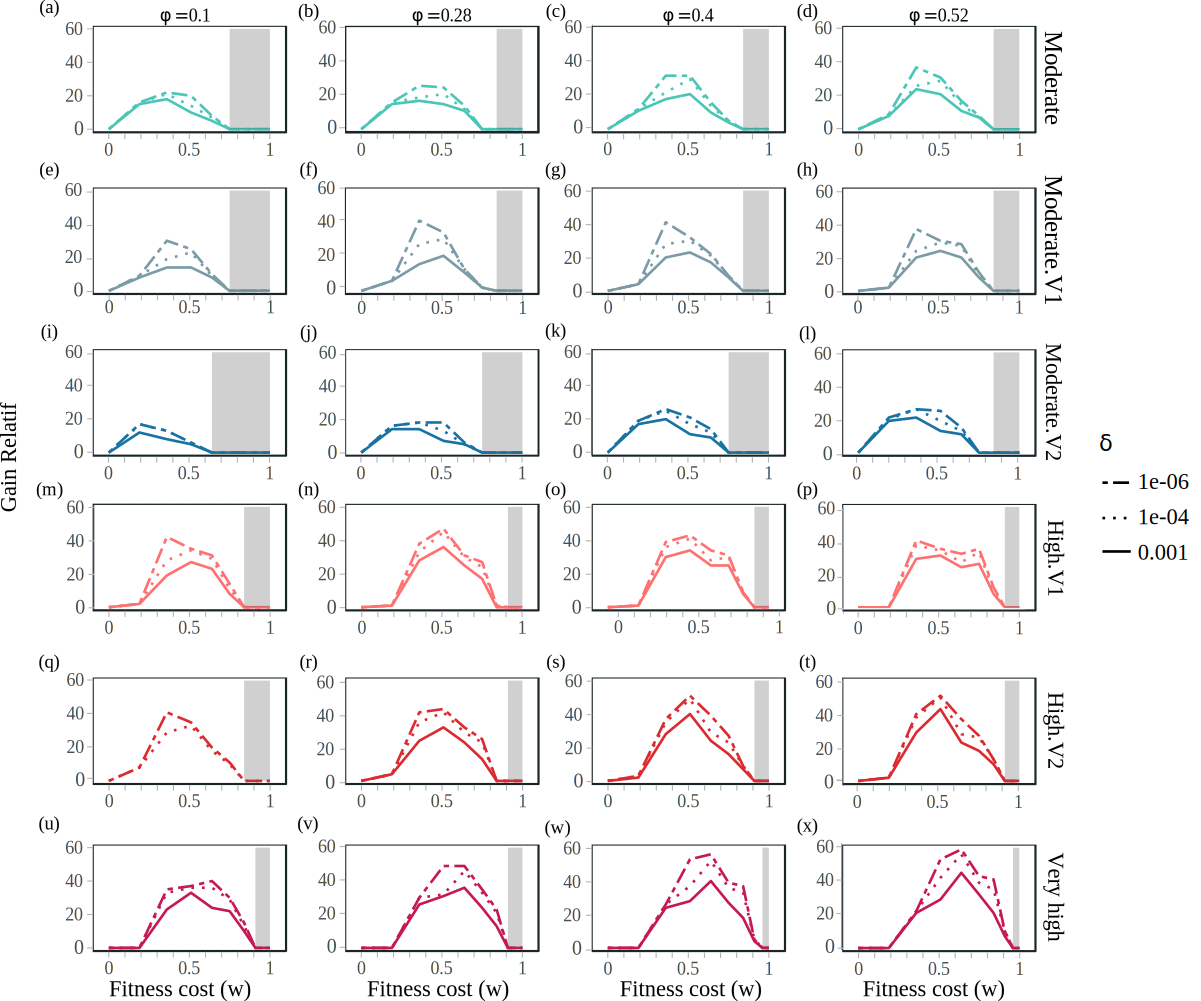
\includegraphics[width=1\linewidth]{Gain_all_sce_phi.pdf}
			\caption[Gain relatif  
			en fonction de 6 scénarios épidémiologique, du coût de fitness efficace, la fréquence de l'émergence 
			d'avirulents à virulents et la survie intersaison.]{Représentation graphique du gain pour 6 scénarios 
			épidémiologiques en fonction du coût de fitness efficace ($w$), la fréquence de l'émergence d'avirulents à 
			virulents ($\delta$) et la survie des nématodes entre les saisons ($\phi$). La zone grise représente
			la zone de durabilité.}
		\label{survie_annexe} 
		\end{figure}



